\chapter{MicroRTS Environment Stack}
\label{chap:python_bridge}

The MicroRTS engine runs on the Java Virtual Machine (JVM) while the RL agent runs in Python. This chapter describes the environment stack that bridges them. Section~\ref{sec:java-python_bridge} details the Java–Python bridge and the per-step interaction cycle. Sections~\ref{sec:obs-encoding} to~\ref{sec:reward-functions} then specify the three signals exchanged through this bridge: the observation tensor, the factored action space with its masking, and the reward signal. Section~\ref{sec:envs} introduces the vectorized environments that orchestrate parallel games, and Section~\ref{sec:wrappers} the composable wrappers that augment them at training time. The implementation builds on Gym-$\mu$RTS~\cite{huangGym$m$RTSAffordableFull2021} with substantial modifications. Figure~\ref{fig:bridge-architecture} gives the resulting data flow.

\begin{figure}[!ht]
    \centering
    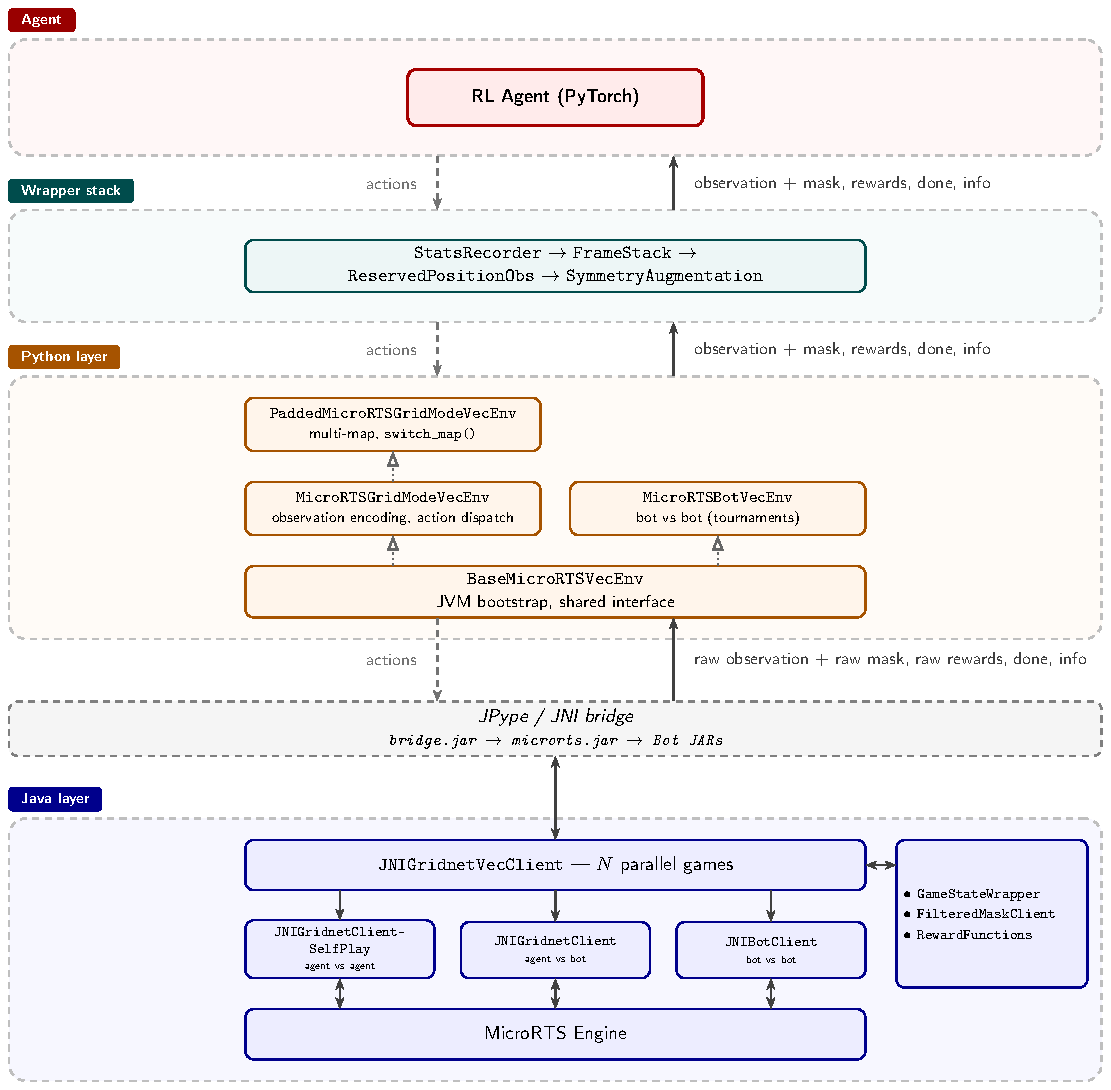
\includegraphics[width=0.88\linewidth]{chapters/07_env_stack/figures/bridge_architecture.pdf}
    \caption[Java–Python training bridge stack]{Full stack of the Java--Python training bridge, from game engine to RL agent. Read bottom to top: the \hlc{blue!7}{Java layer} executes the game simulation, the \hlc{black!4}{JPype bridge} batches communication, the \hlc{orange!8}{Python environment} exposes Gym-compatible observations and actions, \hlc{teal!7}{wrappers} transform the training signal, and the \hlc{red!8}{RL agent} consumes the final tensors.}
    \label{fig:bridge-architecture}
\end{figure}

\section{Java-Python Bridge}
\label{sec:java-python_bridge}

\subsection{\emph{JPype} Integration}
\label{subsec:jvm-integration}

Communication between the two languages happens in-process through \emph{JPype}, which embeds a JVM inside the Python process via the Java Native Interface (JNI). A critical constraint is that the JVM can be started exactly once per process, which shapes the design of the entire stack: all environments, parallel games, and map switches must share a single JVM instance. This rules out a simple design where each environment independently starts and stops its own JVM. Within the shared JVM, a \emph{vectorized client} manages $N$ parallel game instances as a single object. Each call to its reset, step, and mask-extraction methods operates on all $N$ games simultaneously and returns batched arrays. This design minimizes JNI crossing overhead: rather than $N$ separate Java calls per step, a single call processes the entire batch. The same client supports three game modes that can coexist within one batch: \emph{self-play} (the agent controls both sides via paired environments), \emph{RL-vs-bot} (the agent vs a Java AI), and \emph{bot-vs-bot} (two Java AIs, used exclusively for tournaments and producing no observations).

\subsection{End-to-End Step Cycle}
\label{subsec:full-step-pipeline}

A complete step cycle traverses the full stack as follows:

\paragraph*{1. Get action masks:} Python requests the action masks from the vectorized client, which returns a binary tensor of shape $(N, H, W, 1 + 78)$. The first channel is the \emph{source unit mask}, marking cells that contain a controllable unit; the remaining 78~channels (Table~\ref{tab:action-space}) mask individual action components. Python separates the source unit mask and reshapes the remaining channels to $(N, H{\times}W, 78)$.

\paragraph*{2. Agent decision:} the neural network maps the $(N, H, W, C)$ observation tensor (Section~\ref{sec:obs-encoding}) to $78$-dimensional per-cell logits structured by the action representation (Section~\ref{sec:action-space}); the $(N, H{\times}W, 78)$ mask filters these into seven masked categoricals per cell, from which actions are sampled, yielding an $(N, H{\times}W, 7)$ tensor.

\paragraph*{3. Action dispatch:} Python keeps only the actions for cells containing controllable units (source unit mask), prepends each cell's grid index, and dispatches the result to Java. The bridge converts each entry into an in-game command and assigns the default \emph{None} to idle units.

\paragraph*{4. Game step:} the Java client advances all $N$ games by one tick, executing both the RL agent's actions (received from Python) and the bot AIs' actions (computed internally). It returns raw observations, raw masks, per-reward-function values (Section~\ref{sec:reward-functions}), done flags, and info dictionaries. When a game terminates (or exceeds the maximum step limit), the client performs an \emph{auto-reset}\footnote{Auto-reset records the terminal signals, resets the game to its initial state, and returns the next observation alongside the terminal outcome.}.

\paragraph*{5. Post-processing:} observations are encoded into the agent's input format, rewards are combined via a weighted sum (Section~\ref{sec:reward-functions}), done flags trigger episode-end handling (player alternation, map cycling, self-play pair synchronization), and the cycle repeats.

\section{Observation Encoding}
\label{sec:obs-encoding}

\begin{table}[!p]
\centering
\small

%%% TABLE 1
\caption[Standard observation encoding (29 channels)]{Standard observation encoding ($C = 29$ channels).}
\label{tab:standard-obs}
\begin{tabularx}{\textwidth}{p{3.2cm}p{4.5cm}Xp{1.5cm}}
\toprule
\textbf{Feature} & \textbf{Classes} & \textbf{Encoding} & \textbf{Channels} \\
\midrule
Hit points        & \{0, 1, 2, 3, $\geq 4$\}             & one-hot clipped & 5 \\
Resources carried & \{0, 1, 2, 3, $\geq 4$\}             & one-hot clipped & 5 \\
Owner             & \{neutral, self, opponent\}           & one-hot & 3 \\
Unit type         & $\mathcal{K} \cup \{\text{empty}\}$  & one-hot & 7+1 \\
Current action    & $\mathcal{A}$                        & one-hot & 6 \\
Terrain           & \{passable, wall\}                   & one-hot & 2 \\
\midrule
\textit{Optional: visibility}\textsuperscript{$\dagger$} & \{visible, explored\}    & binary & 2 \\
\midrule
\textbf{Total}    &                                      &         & \textbf{29--31} \\
\bottomrule
\multicolumn{4}{@{}p{\textwidth}}{\scriptsize \textsuperscript{$\dagger$}Only relevant under fog-of-war, which is not used in this thesis. These channels are excluded from all experiments ($C = 29$).} \\
\end{tabularx}

\vspace{4em}

%%% TABLE 2
\caption[Extended observation encoding (73 channels)]{Extended observation encoding ($C = 73$ channels).}
\label{tab:extended-obs}
\begin{tabularx}{\textwidth}{p{3.4cm}p{3.5cm}Xp{2cm}}
\toprule
\textbf{Feature} & \textbf{Classes} & \textbf{Encoding} & \textbf{Channels} \\
\midrule
Hit points        & $[0, 10]$                                    & continuous (normalized) & 1 \\
Resources         & $[0, 40]$                                    & continuous (normalized) + threshold ($\geq 1$) & 2 \\
Owner             & \{neutral, self, opponent\}                  & one-hot & 3 \\
Unit type         & $\mathcal{K} \cup \{\text{empty, pending}\}$ & one-hot & 7+2 \\
Current action    & $\mathcal{A}$                                & one-hot & 6 \\
Move direction    & $\mathcal{D} \cup \{\text{idle}\}$           & one-hot & 4+1 \\
Harvest direction & $\mathcal{D} \cup \{\text{idle}\}$           & one-hot & 4+1 \\
Return direction  & $\mathcal{D} \cup \{\text{idle}\}$           & one-hot & 4+1 \\
Produce direction & $\mathcal{D} \cup \{\text{idle}\}$           & one-hot & 4+1 \\
Produce type      & $\mathcal{K} \cup \{\text{idle}\}$           & one-hot & 7+1 \\
Attack direction  & $\mathcal{D} \cup \{\text{idle, ranged}\}$   & one-hot & 4+2 \\
ETA\textsuperscript{$\dagger$}  & $[0, 255]$                            & continuous (normalized) + thresholds ($\geq 5$, $\geq 10$) & 3 \\
Terrain           & \{passable, wall\}                           & binary & 1 \\
\midrule
\multicolumn{3}{l}{\textit{Per-cell subtotal}} & 59 \\
\midrule
Player resources (self)\textsuperscript{$\ddagger$} & $[0, +\infty[$ & continuous (normalized) + 6 thresholds\textsuperscript{$\S$} & 7 \\
Player resources (opp.)\textsuperscript{$\ddagger$} & $[0, +\infty[$ & continuous (normalized) + 6 thresholds\textsuperscript{$\S$} & 7 \\
\midrule
\textit{Optional: visibility}\textsuperscript{$\|$} & \{visible, explored\}     & binary & 2 \\
\midrule
\textbf{Total}    &                                              &  & \textbf{73--75} \\
\bottomrule
\multicolumn{4}{p{\textwidth}}{%
  \footnotesize
  \textsuperscript{$\dagger$}~Estimated Time of Arrival (ETA): remaining game ticks before the current action completes; clamped to $[0, 255]$ and normalized to $[0, 1]$.\newline
  \textsuperscript{$\ddagger$}~Normalized by 32; values above are treated as equivalent. These global resource channels are scalar values broadcast identically to every cell.\newline
  \textsuperscript{$\S$}~Thresholds at $\geq 1, 2, 3, 5, 10, 32$, matching unit production costs: Worker~(1), Light/Ranged~(2), Heavy~(3), Barracks~(5), Base~(10).\newline
  \textsuperscript{$\|$}~Only relevant under fog-of-war, which is not used in this thesis. These channels are excluded from all experiments ($C = 73$).
} \\
\end{tabularx}
\end{table}

The Python layer supports two observation encodings, both producing a spatial tensor of shape $(H, W, C)$ by stacking encoded planes along the channel axis. The \emph{standard} encoding, inherited from Gym-$\mu$RTS~\cite{huangGym$m$RTSAffordableFull2021}, represents every feature as a one-hot category, yielding a binary tensor with $C=29$. The \emph{extended} encoding, adapted from RAISocketAI~\cite{goodfriendCompetitionWinningDeep2024}, combines continuous values, threshold flags, and one-hot fields, reaching $C=73$ and exposing information the binary scheme cannot represent.

Following Gym-$\mu$RTS convention, unit ownership is encoded from the observing player's perspective: the network always sees its own units identically, regardless of which side it controls.

\paragraph*{Standard encoding ($C = 29$ channels).}

The standard encoding uses the \code{GameState} class to extract 6 raw features per cell. Table~\ref{tab:standard-obs} details the resulting channels and Figure~\ref{fig:obs-encoding-viz} illustrates the encoding on three example cells.

\begin{figure}[!htb]
\centering
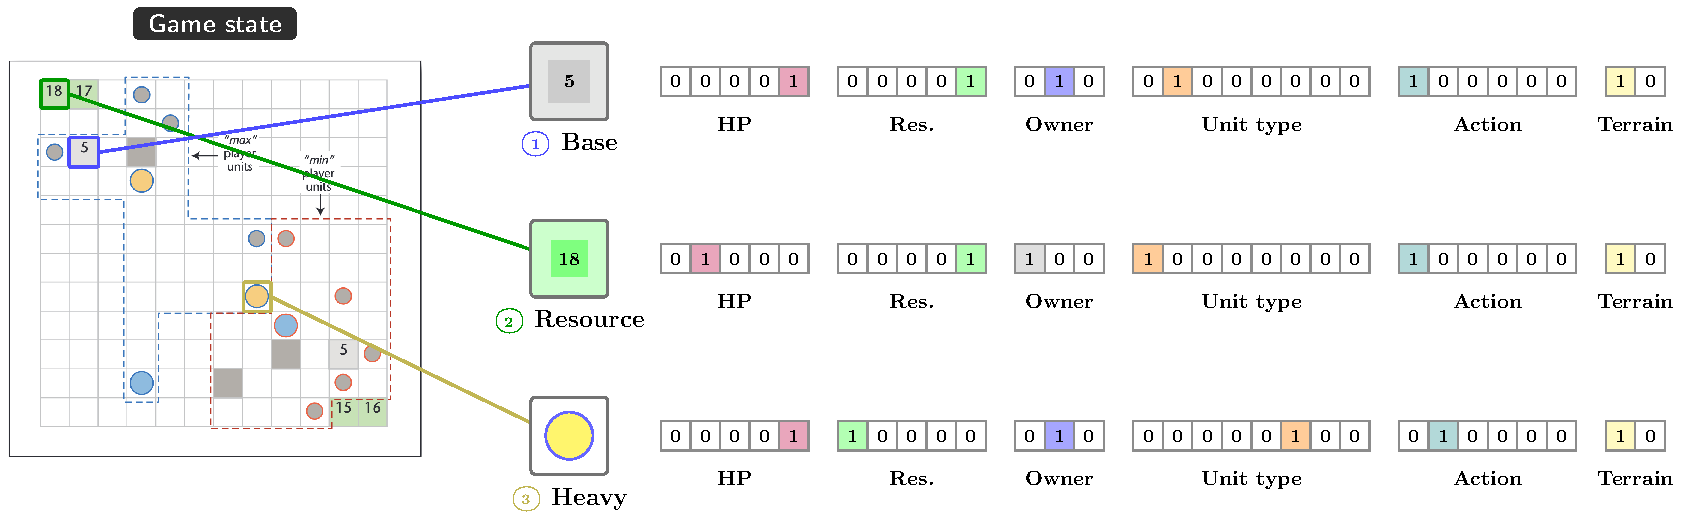
\includegraphics[width=\linewidth]{chapters/07_env_stack/figures/obs_encoding_viz.pdf}
\caption[Standard observation encoding (example cells)]{Standard observation encoding: three cells from a game state and their encodings. Each cell of the $H{\times}W$ grid is encoded independently, producing a tensor of shape $(H, W, 29)$.}
\label{fig:obs-encoding-viz}
\end{figure}

\paragraph*{Extended encoding ($C = 73$ channels).}

The extended encoding uses \code{GameStateWrapper} to extract 13 features per cell, complemented by global resource counts broadcast identically to every cell. Table~\ref{tab:extended-obs} details the full encoding.

\section{Action Space and Masking}
\label{sec:action-space}

The agent outputs per-cell action logits using the GridNet factored action representation. For each of the $H{\times}W$ grid cells, the network produces logits over seven components (Table~\ref{tab:action-space}).

\begin{table}[!htb]
\centering
\caption[Factored action space per grid cell]{Factored action space per grid cell.}
\label{tab:action-space}
\begin{tabularx}{\textwidth}{p{3.5cm}p{4.8cm}Xp{1.5cm}}
\toprule
\textbf{Component} & \textbf{Classes} & \textbf{Encoding} & \textbf{Channels} \\
\midrule
Action type       & $\mathcal{A}$  & discrete & 6 \\
Move direction    & $\mathcal{D}$  & discrete & 4 \\
Harvest direction & $\mathcal{D}$  & discrete & 4 \\
Return direction  & $\mathcal{D}$  & discrete & 4 \\
Produce direction & $\mathcal{D}$  & discrete & 4 \\
Produce type      & $\mathcal{K}$  & discrete & 7 \\
Attack target     & $7{\times}7$ relative grid\textsuperscript{$\dagger$} & discrete & 49 \\
\midrule
\multicolumn{3}{l}{\textbf{Total per cell}} & \textbf{78} \\
\bottomrule
\multicolumn{4}{@{}p{\textwidth}}{\scriptsize
  \textsuperscript{$\dagger$}A $7{\times}7$ grid centered on the acting unit. Index $i = (3 + \Delta y) \times 7 + (3 + \Delta x)$, where $(\Delta x, \Delta y)$ is the relative offset to the target. Index 24 corresponds to the unit's own cell.
} \\
\end{tabularx}
\end{table}

The action space is defined as a \code{MultiDiscrete} of size $H{\times}W{\times}78$~\cite{huangGym$m$RTSAffordableFull2021, 
brockmanOpenAIGym2016}. At each timestep, the environment provides a binary mask of shape $(N, H{\times}W, 78)$ indicating valid actions~\cite{huangCloserLookInvalid2022}: before sampling, invalid logits are set to $-10^8$, zeroing their softmax probability. Without this masking, agents would waste most of their exploration budget on illegal actions. Independent per-cell masking, however, still allows a subtle failure mode known as \emph{destination collision}: two units moving or producing into the same cell within a single step, causing one action to fail silently. Inspired by RAISocketAI~\cite{goodfriendCompetitionWinningDeep2024}, \emph{filtered masking} tracks destinations of in-progress actions and excludes those cells before generating masks for newly idle units. Figure~\ref{fig:action-masking-viz} illustrates the improvement.

\begin{figure}[!ht]
\centering
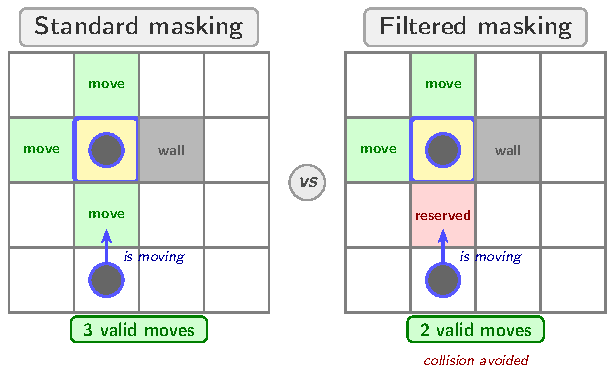
\includegraphics[width=0.65\linewidth]{chapters/07_env_stack/figures/action_masking_viz.pdf}
\caption[Standard vs destination-aware filtered masking]{\emph{Standard} vs \emph{destination-aware} filtered masking. Left: the selected worker (yellow cell) has three valid moves. Right: cell (2,2) is blocked because the other worker is already moving there.}
\label{fig:action-masking-viz}
\end{figure}

\vspace{-1.5em}

\section{Reward Functions}
\label{sec:reward-functions}

The scalar reward at each step is $r_{t+1} = \mathbf{w}^\top \mathbf{r}_{t+1}$ (Section~\ref{subsec:microrts_mdp}), where $\mathbf{r}_{t+1}$ is a $9$-component raw reward vector~\cite{vanseijenHybridRewardArchitecture2017} and $\mathbf{w}$ the weight vector. Table~\ref{tab:reward-functions} lists the nine components: a single sparse Win/Draw/Loss signal at game termination, plus eight dense rewards triggered by intermediate game events. The terminal signal alone yields too few learning samples over the thousands of timesteps of a typical game, so these shaped rewards~\cite{ngPolicyInvarianceReward1999} densify the feedback, with default weights set so that the terminal outcome still dominates the cumulative return.

\begin{table}[!ht]
\centering
\caption[Reward functions available during training]{Reward functions available during training.}
\label{tab:reward-functions}
\small
\begin{tabularx}{\textwidth}{p{3.2cm}Xp{1.5cm}p{2cm}}
\toprule
\textbf{Reward function} & \textbf{Signal description} & \textbf{Type} & \textbf{Default weight} \\
\midrule
Win/Draw/Loss         & $+1$ on win, $0$ on draw, $-1$ on loss                                          & sparse & $10.0$ \\
Resource gathering    & $+1$ per resource unit delivered to a base                                      & dense  & $1.0$ \\
Worker production     & $+1$ per worker trained at a base                                               & dense  & $1.0$  \\
Light production      & $+1$ per light unit trained at barracks                                         & dense  & $4.0$  \\
Heavy production      & $+1$ per heavy unit trained at barracks                                         & dense  & $4.0$  \\
Ranged production     & $+1$ per ranged unit trained at barracks                                        & dense  & $4.0$  \\
Base construction     & $+1$ per base built by a worker                                                 & dense  & $0.1$  \\
Barracks construction & $+1$ per barracks built by a worker                                             & dense  & $0.1$  \\
Attack damage         & $+1$ per attack action issued on an enemy                                       & dense  & $1.0$  \\
\bottomrule
\end{tabularx}
\end{table}

\section{Vectorized Environments}
\label{sec:envs}

The original Gym-$\mu$RTS codebase provided a single monolithic environment class handling all use cases. It is refactored here into three specialized classes built on a shared base, separating bot-only evaluation from RL training and adding support for the extended encoding, filtered masking, self-play, multi-map training, and side alternation introduced in Sections~\ref{sec:obs-encoding} to~\ref{sec:reward-functions}.

\subsection{Environment Classes}
\label{subsec:env-classes}

Three vectorized environment classes specialize the per-step logic:

\paragraph*{Bot-vs-bot environment.} Runs $N$ parallel games between two Java AIs and is used exclusively for round-robin tournament evaluation. No observation tensor is returned; only the win/draw/loss outcome is collected for each game.

\paragraph*{Agents environment.} The main training environment. It manages $N_\text{sp} + N_\text{bot}$ parallel games combining self-play pairs (the agent controls both sides via a shared underlying game instance) and RL-vs-bot games (the agent vs a Java AI). Bot games start on a configured side (P0 or P1) and optionally alternate sides at episode end to balance the experience distribution. The per-step data flow follows the pipeline of Section~\ref{subsec:full-step-pipeline}.

\paragraph*{Padded environment.} Extends the agents environment with zero-padding to enable multi-map training without restarting the JVM (Section~\ref{subsec:padding} below).

\subsection{Padding for Multi-Map Training}
\label{subsec:padding}

A neural network expects a fixed input shape throughout training, but MicroRTS maps have different dimensions. RAISocketAI~\cite{goodfriendCompetitionWinningDeep2024} rewrote the entire Java--Python bridge to natively dispatch on map shape at runtime. An alternative would project every map to a common fixed-size representation, but this would discard the per-cell spatial structure on which the GridNet factored action representation depends (Section~\ref{sec:action-space}). Given the complexity of the first approach (compounded by the JVM single-startup constraint, Section~\ref{subsec:jvm-integration}) and the information loss of the second, a simpler approach is adopted here: padding all observations to a fixed maximum size, as illustrated in Figure~\ref{fig:padded-env}.

\begin{figure}[!ht]
\centering
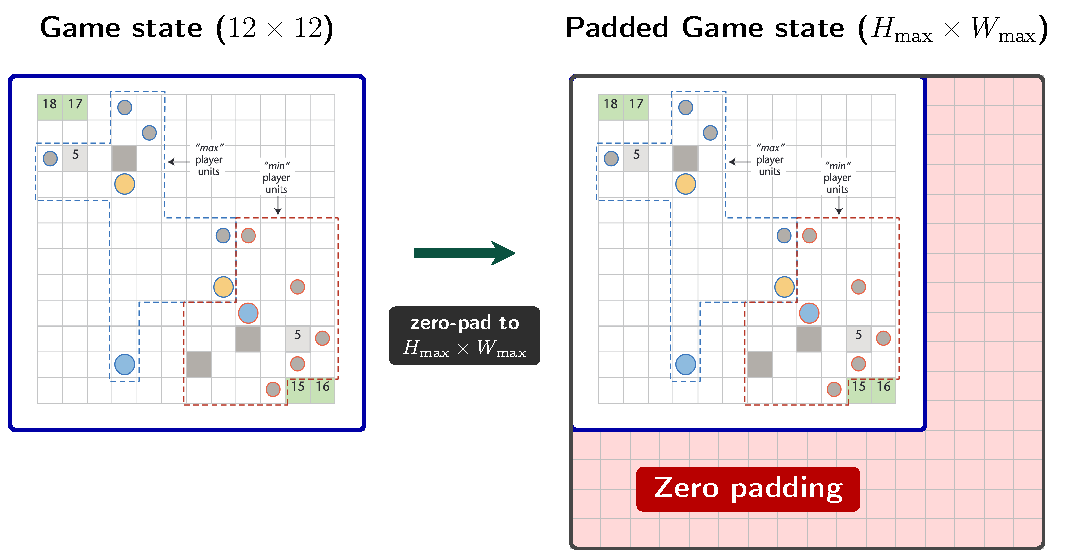
\includegraphics[width=0.75\linewidth]{chapters/07_env_stack/figures/padded_env.pdf}
\caption[Padded environment for multi-map training]{Padded environment for multi-map training. The game state (left) is embedded into a fixed-size tensor sized to the largest map in the training pool (right). Padded cells contain zeros and receive all-zero action masks, preventing the agent from acting outside the actual map boundaries.}
\label{fig:padded-env}
\end{figure}

The padded environment maintains two sets of dimensions: the \emph{actual} map size $(H, W)$ used by the Java engine, and a fixed \emph{padded} size $(H_\text{max}, W_\text{max})$ seen by the agent. Observations are zero-padded from $(N, H, W, C)$ to $(N, H_\text{max}, W_\text{max}, C)$, with padded cells appearing as empty terrain. Action masks follow the same treatment, so that padded cells receive all-zero masks and the agent cannot act on them. Actions go in the reverse direction: cropped to the actual $(H, W)$ region before being dispatched to Java. This approach preserves a uniform tensor shape across all maps but introduces computational overhead proportional to the padded-to-actual area ratio, since convolutional layers still process the padded cells (the action mask only applies at output time). For instance, a $16{\times}16$ map padded to $64{\times}64$ wastes $93.75$\% of the spatial computation on empty cells.

Together, these properties enable the central capability that motivated the padded environment: training on multiple maps within a single run. The active map can be switched at any time without restarting the JVM, and since the padded dimensions remain fixed, the network architecture does not change across maps. The base environment classes could not support this; each map size would have required its own network and a separate training run.

\section{Composable Wrappers}
\label{sec:wrappers}

A key design principle separates \emph{environments} from \emph{wrappers}. The vectorized environment classes handle the Java interface, game simulation, and core observation/action encoding. Most additional processing is implemented as composable Gym wrappers that sit between the environment and the agent, ensuring each wrapper can be toggled independently via CLI flags.

Four wrappers are available, composed in a fixed order:
\begin{enumerate}
    \item \textbf{\code{StatsRecorder}.} Accumulates each of the nine raw reward components separately over an episode, as both raw and discounted ($\gamma^t \cdot r_{t+1}$) sums. The cumulative per-component values are emitted at episode termination for monitoring tools such as TensorBoard.
    
    \item \textbf{\code{FrameStack}.} Stacks the last $k$ observations along the channel axis, producing tensors of shape $(H, W, k \cdot C)$~\cite{mnihHumanlevelControlDeep2015}. This gives the convolutional encoder access to temporal patterns (unit movement, production sequences) without recurrence. Action masks remain unstacked since they depend only on the current game state.
    
    \item \textbf{\code{ReservedPositionObs}.} Companion to destination-aware filtered masking (Section~\ref{sec:action-space}): the mask filters out reserved cells but does not reveal them to the agent. This wrapper appends a binary observation channel ($C \to C + 1$) flagging cells reserved by pending actions, letting the network plan around spatial conflicts.
    
    \item \textbf{\code{SymmetryAugmentation}.} Exploits the spatial symmetry of MicroRTS maps. At each episode start, each environment is assigned one of four random flip modes (identity, horizontal flip, vertical flip, or $180^\circ$ rotation). Observations and action masks are transformed accordingly; actions are unflipped before being dispatched to the engine. Direction-dependent components (move, harvest, return, produce directions, and the $7{\times}7$ attack target grid) are remapped consistently. This effectively quadruples the diversity of training positions without additional environment interaction~\cite{laskinReinforcementLearningAugmented2020}. It is applied only during training, never during evaluation, to ensure deterministic and unbiased assessment.
\end{enumerate}